\documentclass[12pt]{article}
\usepackage[margin=1.25in]{geometry}
\usepackage{amsmath, amssymb}
\usepackage{array}
\usepackage{gensymb}
\usepackage{tikz, pgfplots}
\usetikzlibrary{shapes, arrows, positioning, plotmarks}
\pgfplotsset{width=10cm,compat=1.9}

\begin{document}
    \begin{center}
        {\large Reciprocal Functions}
    \end{center}

    Parent function: \(f(x)=\frac{1}{x}\)

    Standard form: \(f(x)=\frac{a}{x-h}+k\)
    
    \begin{center}
        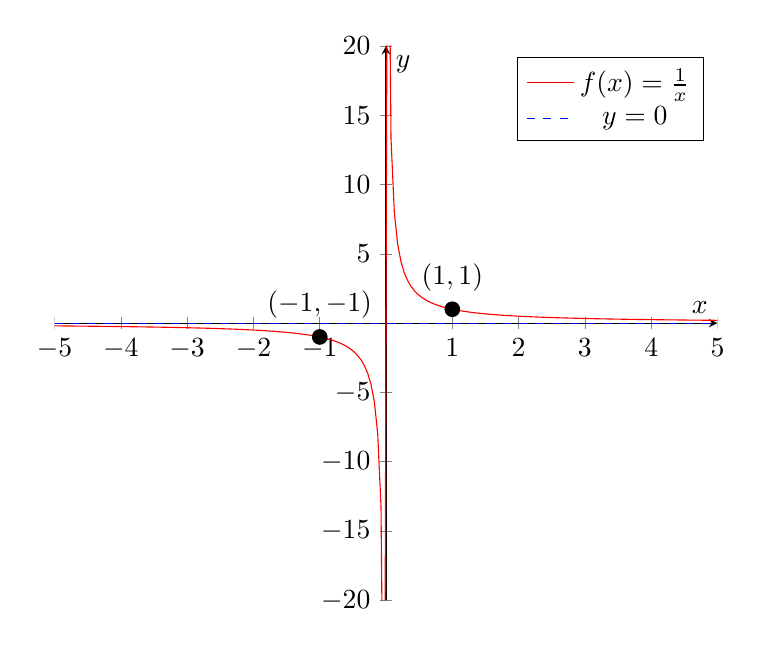
\begin{tikzpicture}
            \begin{axis}[
                    axis lines = middle,
                    xlabel = \(x\),
                    ylabel = \(y\),
                    xtick distance = 1,
                    ytick distance = 5,
                    ymin = -20,
                    ymax = 20,
                ]
                \addplot[color = red, samples = 200]{1 / x};
                \addlegendentry{\(f(x)=\frac{1}{x}\)}
                \node[label={90:{\((1,1)\)}},circle,fill,inner sep=2pt] at (axis cs:1,1) {};
                \node[label={90:{\((-1,-1)\)}},circle,fill,inner sep=2pt] at (axis cs:-1,-1) {};

                \addplot[color = blue, style = dashed]{0};
                \addlegendentry{\(y=0\)}
            \end{axis}
        \end{tikzpicture}
    \end{center}

    Reciprocal functions always have 2 or more asymptotes: 1 or more vertical asymptote, and a horizontal \textbf{or} slant asymptote. Should \(a\) remain a constant, the horizontal asymptote is at \(y=k\), and the vertical asymptotes are at \(x=n\), where \(n\) is all values of \(x\) that make the expression on the denominator equal 0.

    Some examples:

    \begin{center}
        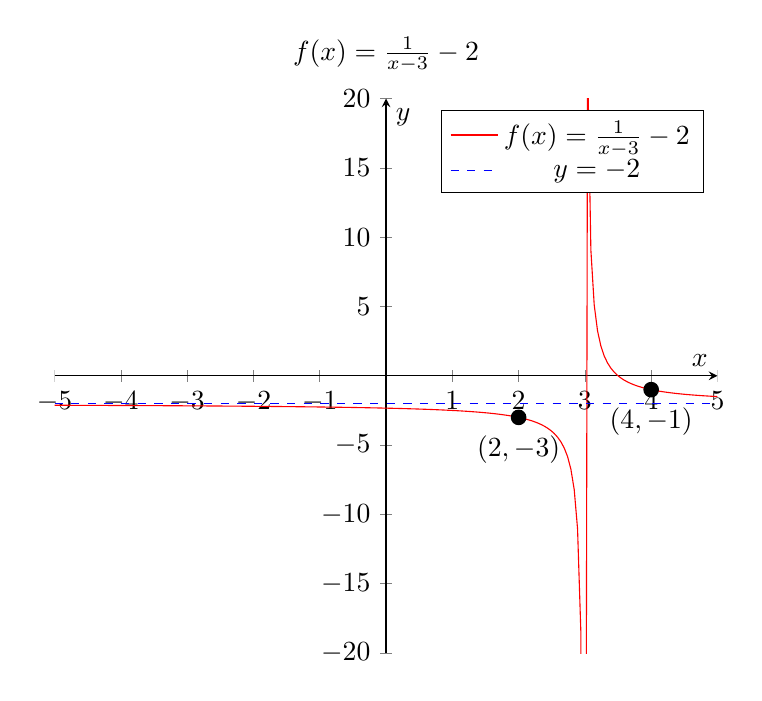
\begin{tikzpicture}
            \begin{axis}[
                axis lines = middle,
                xlabel = \(x\),
                ylabel = \(y\),
                xtick distance = 1,
                ytick distance = 5,
                ymin = -20,
                ymax = 20,
                title = {\(f(x)=\frac{1}{x-3}-2\)}
            ]
                \addplot[color = red, samples = 200]{(1 / (x - 3)) - 2};
                \addlegendentry{\(f(x)=\frac{1}{x-3}-2\)}
                \node[label={270:{\((2,-3)\)}},circle,fill,inner sep=2pt] at (axis cs:2,-3) {};
                \node[label={270:{\((4,-1)\)}},circle,fill,inner sep=2pt] at (axis cs:4,-1) {};

                \addplot[color = blue, style = dashed]{-2};
                \addlegendentry{\(y=-2\)}
            \end{axis}
        \end{tikzpicture}
    \end{center}

    Here, \(h=3\), so the function is translated 3 units right, so the vertical asymptote is at \(x=3\). Similarly, \(k=-2\), so the function is translated 2 units down, so the horizontal asymptote is at \(y=-2\).

    \begin{center}
        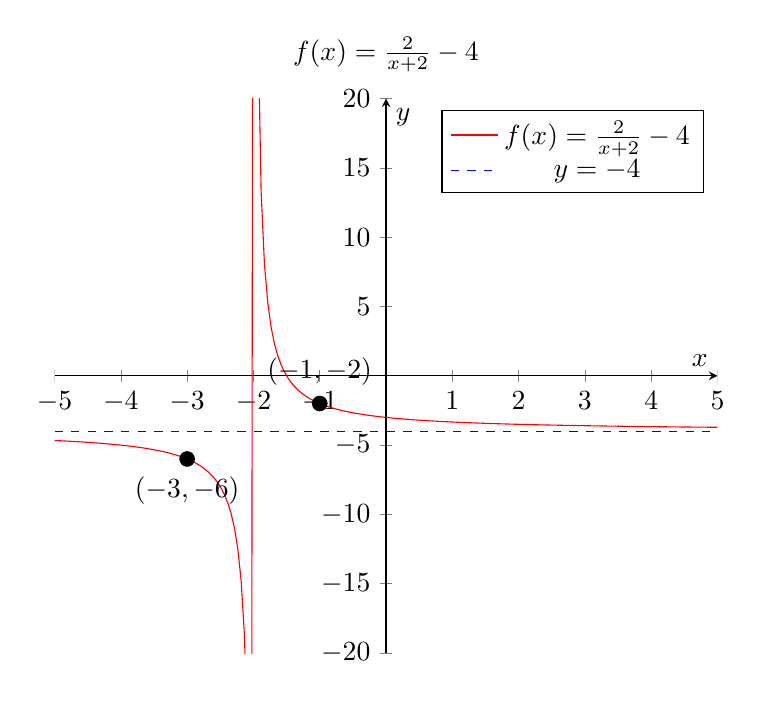
\begin{tikzpicture}
            \begin{axis}[
                axis lines = middle,
                xlabel = \(x\),
                ylabel = \(y\),
                xtick distance = 1,
                ytick distance = 5,
                ymin = -20,
                ymax = 20,
                title = {\(f(x)=\frac{2}{x+2}-4\)}
            ]
                \addplot[color = red, samples = 200]{(2 / (x + 2)) - 4};
                \addlegendentry{\(f(x)=\frac{2}{x+2}-4\)}
                \node[label={270:{\((-3,-6)\)}},circle,fill,inner sep=2pt] at (axis cs:-3,-6) {};
                \node[label={90:{\((-1,-2)\)}},circle,fill,inner sep=2pt] at (axis cs:-1,-2) {};

                \addplot[color = blue, style = dashed]{-4};
                \addlegendentry{\(y=-4\)}
            \end{axis}
        \end{tikzpicture}
    \end{center}

    Here, \(h=-2\), so the function is translated 2 units left, so the vertical asymptote is at \(x=-2\). Similarly, \(k=-4\), so the function is translated 4 units down, so the horizontal asymptote is at \(y=-4\).

    There are a few special cases for the horizontal asymptote where \(a\) is a polynomial rather than a constant.\\

    \textbf{Should the degree in the numerator be less than in the denominator,} the horizontal asymptote will be at \(y=0\)\\

    \textbf{Should the degree in the numerator be equal to that in the denominator,} the horizontal asymptote will be at \(y=n\), where \(n\) is the quotient of the greatest-degree coefficients of the numerator and denominator.\\
    For example, given the function \(f(x)=\frac{-15x+10}{3x-33}\), we can divide 6 by 3 to find that the horizontal asymptote of \(f(x)\) is at \(y=-5\).\\

    \begin{center}
        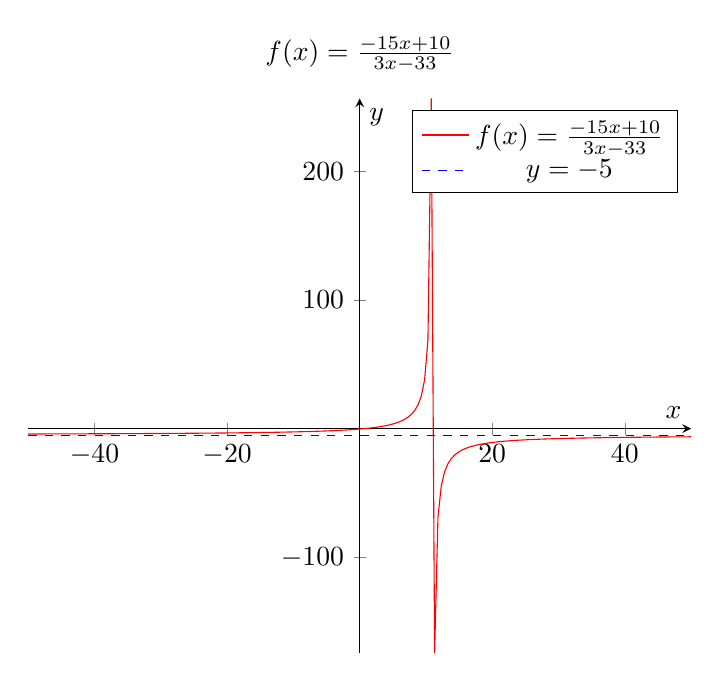
\begin{tikzpicture}
            \begin{axis}[
                axis lines = middle,
                xlabel = \(x\),
                ylabel = \(y\),
                title = {\(f(x)=\frac{-15x+10}{3x-33}\)}
            ]
                \addplot[color = red, samples = 200, domain = -50:50]{((-15 * x)  + 10) / ((3 * x) - 33)};
                \addlegendentry{\(f(x)=\frac{-15x+10}{3x-33}\)}
                \addplot[color = blue, style = dashed, domain = -50:50]{-5};
                \addlegendentry{\(y=-5\)}
            \end{axis}
        \end{tikzpicture}
    \end{center}

    \textbf{Should the degree in the numerator be greater than in the denominator,} there is not a horizontal asymptote, but a slant asymptote. The slant asymptote will be at \(y=nx\), where \(n\) is the result of long-dividing the numerator and denominator and excluding the remainder.\\
    For example, given the function \(f(x)=\frac{2x^2-4x+5}{x+2}\), we can do long division to find that \(\frac{2x^2-4x+5}{x+2}=2x-8+\frac{21}{x+2}\). From this, we can derive that the slant asymptote of \(f(x)\) is \(y=2x-8\).

    \begin{center}
        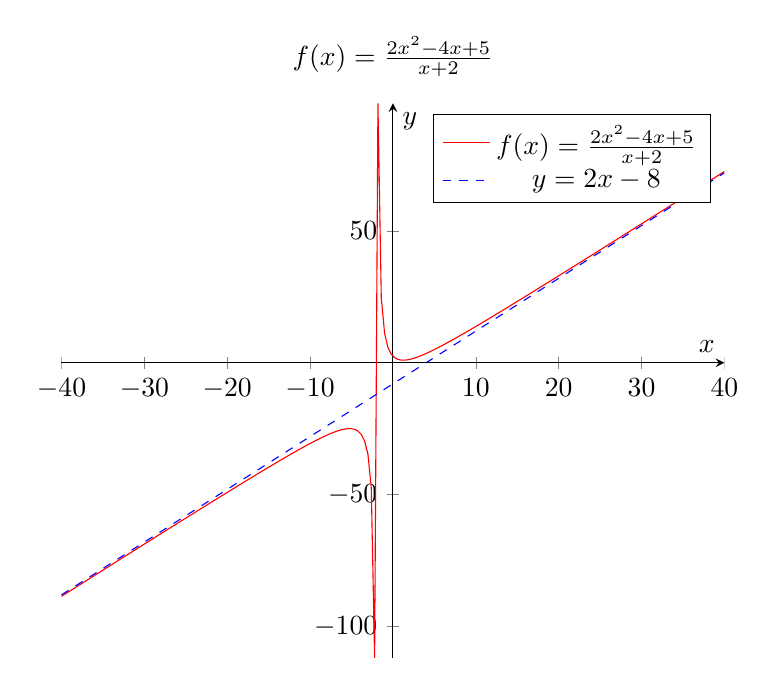
\begin{tikzpicture}
            \begin{axis}[
                axis lines = middle,
                xlabel = \(x\),
                ylabel = \(y\),
                title = {\(f(x)=\frac{2x^2-4x+5}{x+2}\)},
            ]
                \addplot[color = red, samples = 200, domain = -40:40]{((2 * x^2) - (4 * x) + 5) / (x + 2)};
                \addlegendentry{\(f(x)=\frac{2x^2-4x+5}{x+2}\)}
                \addplot[color = blue, style = dashed, domain = -40:40]{(2 * x) - 8};
                \addlegendentry{\(y=2x-8\)}
            \end{axis}
        \end{tikzpicture}
    \end{center}

    And here we can see that this is correct.

    \begin{center}
        {\large The Trigonometric Identities}
    \end{center}

    \noindent The angle sum identities are as follows:
    \begin{itemize}
        \item \(\sin(\alpha\pm\beta)=\sin(\alpha)\cos(\beta)\pm\sin(\beta)\cos(\alpha)\)
        \item \(\cos(\alpha\pm\beta)=\cos(\alpha)\cos(\beta)\mp\sin(\alpha)sin(\beta)\)
        \item \(\tan(\alpha\pm\beta)=\frac{\tan(\alpha)\pm\tan(\beta)}{1\mp\tan(\alpha)\tan(\beta)}\)
    \end{itemize}

    \noindent These ``double'' identities can be derived from the sum identities:
    \begin{itemize}
        \item \(\sin(2\theta)=2\sin(\theta)\cos(\theta)\)
        \item \(\cos(2\theta)=cos^2(\theta)-\sin^2(\theta)=2\cos^2(\theta)-1=1-2\sin^2(\theta)\)
        \item \(\tan(2\theta)=\frac{2\tan(\theta)}{1-\tan^2(\theta)}\)
    \end{itemize}

    \noindent There are also half-angle identities:
    \begin{itemize}
        \item \(\sin(\frac{\theta}{2})=\pm\sqrt{\frac{1-\cos(\theta)}{2}}\)
        \item \(\cos(\frac{\theta}{2})=\pm\sqrt{\frac{1+\cos(\theta)}{2}}\)
        \item \(\tan(\frac{\theta}{2})=\pm\sqrt{\frac{1-\cos(\theta)}{1+\cos(\theta)}}=\frac{1-\cos(\theta)}{\sin(\theta)}=\frac{\sin(\theta)}{1+\cos(\theta)}\)
    \end{itemize}

    \noindent Some other crucial ones:
    \begin{itemize}
        \item \(\sin^2(\theta)+\cos^2(\theta)=1\)
        \item \(\sec^2(\theta)=1+\tan^2(\theta)\)
        \item \(\csc^2(\theta)=1+\cot^2(\theta)\)
    \end{itemize}
\end{document}